\begin{document}
The in order to activate the IR LED correctly it has to driven with a square wave. The generated waveform from the ring oscillator circuit is, however, a distorted sinuisoid. The signal must therefore be transformed into a square wave. This requires the use of a signal conditioner. A Schmitt trigger was chosen to implement the signal condition. 
%% SCHMITT TRIGGER SCHEMATIC HERE
The Schmitt trigger is an positive feedback configuration for a noninverting amplifier. The Schmitt trigger is described most succinctly by its transfer function, seen in Figure \ref{fig:schmitttransfer}.

\begin{figure}[H]
	\centering
	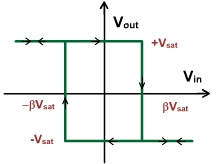
\includegraphics[width=0.6\linewidth]{schmitttransfer}
	\caption[Transfer function of Schmitt Trigger]{Transfer Function of Schmitt Trigger \cite{schmitt}}
	\label{fig:schmitttransfer}
\end{figure}
The Schmitt trigger outputs two discrete voltages, which are set by the reference node at $V_-$. This voltage determines when the output voltage drops to the low or up to its high voltage. The simulated circuit is shown in Figure \ref{fig:signalconditionersimulationschem}.

\begin{figure}[H]
	\centering
	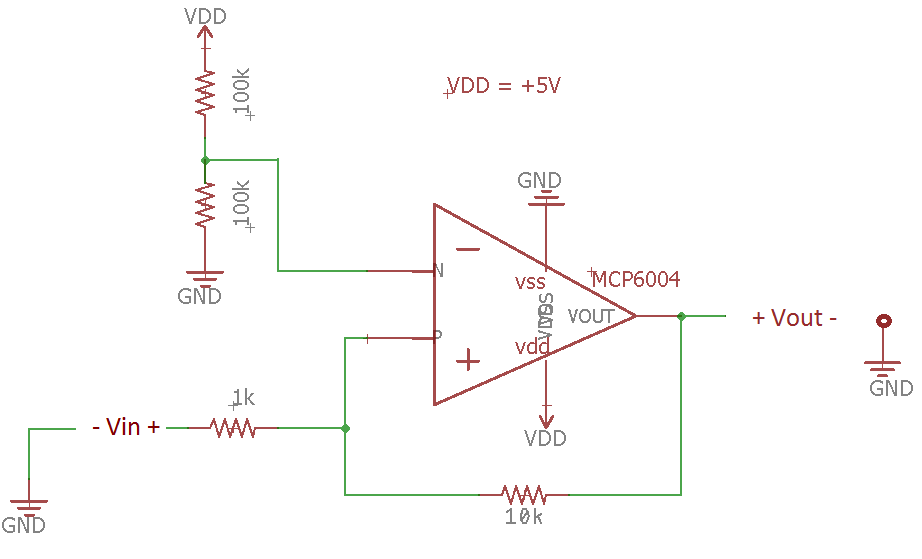
\includegraphics[width=0.6\linewidth]{SignalConditionerSimulationSchem}
	\caption[Simulated signal conditioner circuit]{Simulated signal conditioner circuit}
	\label{fig:signalconditionersimulationschem}
\end{figure}

The input to the signal conditioner is the 5V peak sinuisoid from the ring oscillator. In order to attain a 50\% duty-cycle, the reference voltage should be set to half of the input signal. As a result, the voltage divider at the reference node is a 50/50 voltage divider, resulting in 2.5V at the reference node. The feedback configuration is set to 10$\frac{V}{V}$ to ensure that the output from the signal conditioner is 5V. When the input signal is about the reference voltage, the Schmitt trigger is "high" and when the signal is below the reference voltage the output is "low". This results in an output square wave. The output waveform can be seen in Figure \ref{fig:signalconditionersimulationschem}.

\begin{figure}[H]
	\centering
	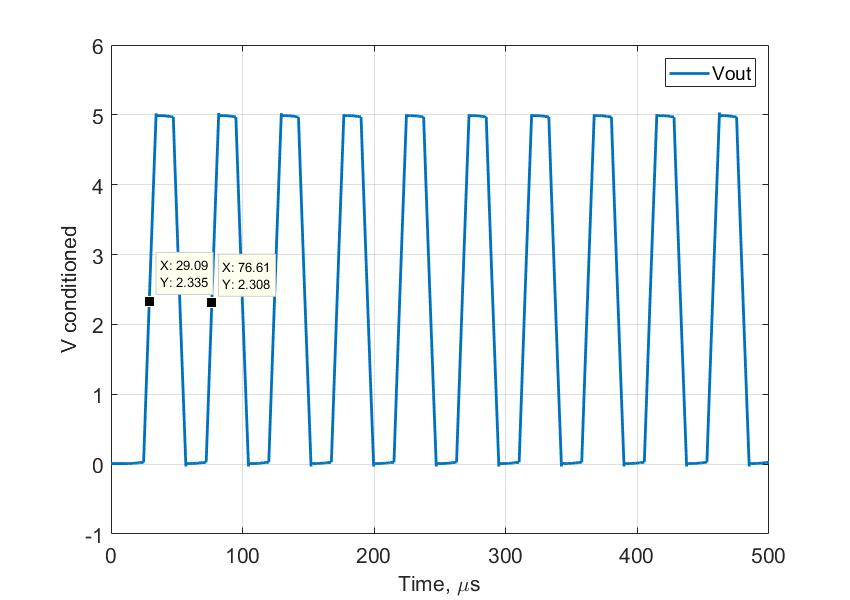
\includegraphics[width=0.6\linewidth]{Vconditioned_sim}
	\caption[Simulated conditioned signal]{Simulated conditioned signal}
	\label{fig:vconditionedsim}
\end{figure}

The output was simulated to have an



\end{document}